\documentclass[12pt]{article}
\usepackage{setspace}
\usepackage[margin = 1.4in]{geometry}
\usepackage{amsfonts, amsmath, amssymb}
\usepackage[none]{hyphenat}
\usepackage{graphicx}

\begin{document}
\begin{titlepage}
   \vspace*{\stretch{1.0}}
   \begin{center}
      \Large\textbf{Genetic Alogrithm for CNN Hyperparametr Optimization}\\
      \vspace*{\stretch{0.3}}
      \large\textit{Tianrui Guo}\\
      \vspace*{\stretch{0.1}}
      \large Department of Applied Mathematics\\
      \vspace*{\stretch{0.1}}
      \large\textit{April 20, 2019}
   \end{center}
   \vspace*{\stretch{2.0}}
\end{titlepage}

\pagebreak
\setlength{\baselineskip}{10mm}
\begin{center}
\LARGE \textbf{Abstract}
\end{center}
In this big data era, we developed many efficient and effective ways to analyze our database. Among various techniques, computer vision is a fancy and important one. One of the most significant technique in modern computer vision is convolutional neural network which is a typical method in deep learning. When we process image classification or image recognition, we inevitably encounter a problem of determine the hyperparamters such as the number of Conv channels, the size of filters or the dimension of the dense layers. The process of finding a set of hyperparameters which can improve the performance of convolutional neural network is known as hyperparameter optimization, and it can be also called as tuning. In this Capstone project we are using genetic algorithm for finding an optimal CNN architecture. When the convolutional neural network goes deeper and more complicated, the number of hyperparameters increases dramatically. In order to increase the performance of tuning, we no longer use manual tuning methods like grid search,  instead we use genetic algorithm which is a kind of random search method for tuning, because we want the optimization algorithm searching automatically in a larger hyperparamter space.  To test the performance of genetic tuning, we implement genetic algorithm on MNIST which is a relative small data set include 60,000 examples in training set and 10,000 examples in test set. If this algorithm performs well in this dataset, we will have possibility to implement it on other significative datasets.\pagebreak
\section{Introduction}
Machine learning is the cutting edge technique in modern data science, and it is dominated by deep neural network. These great inventions enable us have much better performance in data analysis. Inspired by the deep neural network architecture, we obtain a rapid development in computer vision. Computer vision is an cutting edge technique making computer to see visual object and extract information from images and videos in the similar way as human does. Image classification and image recognition are the art-of-state field in computer vision, and they have significant contribution to human face recognition, automatic driving and neural style transfer. In this capstone project, we are using convolutional neural network to train MNIST dataset, and this is a kind of image classification. MNIST dataset is a large database of handwritten digits that is commonly used for training various image processing systems. The examples in MNIST dataset are black and white images of human handwritten digits and they are normalized to fit into a $28 \times 28$ pixel bounding box and anti-aliased, which introduced grayscale levels. Hence, we can encode the images into matrices which have all entries equals to one or zero, this problem is transferred as matrix regression. The framework we use to process image classification of MNIST dataset is convolutional neural network (we called CNN or Conv neural network later). Convolutional neural network (CNN, or ConvNet) is a class of deep neural networks, most commonly applied to analyzing visual imagery. Convolutional networks were inspired by biological mechanism in that the connectivity pattern between neurons resembles the organization of the animal visual cortex. The advantage of CNN of image classification is CNN has a weight-sharing feature. Comparing with fully connected neural networks, CNN has conspicuous fewer parameters which makes CNN extract information from dataset at lower computational cost. \\
~\\
The main purpose of this project is to find an optimal hyperparameter set for CNN framework. In deep learning, a hyperparameter is a parameter whose value is set before the training begins. Different models have different types of hyperparameters, in our CNN model we have filter size, Conv layer channel, pooling size, drop out rate and dense layer size as hyperparameters. Hyperparameters are integers and continuous numbers in our model, leading to mixed-type optimization problems. The choice of hyperparameters can affect the performance of deep neural network significantly. The accuracy and the time required for training process will depend on the hyperparameters we choose. To improve performance of our CNN model, we can apply various tuning methods to find a set of optimal hyperparameters. In this case we are applying genetic algorithm for hyperparameter optimization. Genetic algorithm for CNN tuning is a kind of population based training which is inspired by the process of natural selection. We consider a tuple of hyperparameters as a chromosome of an individual. In our model, we assume every individual has only one chromosome. Since one chromosome represents a tuple of hyperparameters, a gene on the chromosome represents one hyperparameter. If a model has ten hyperparameter, the individual will have one chromosome consists ten genes. For our genetic algorithm, all the individuals in the same generation constitute the whole population. In next section, we will discuss each gene on the chromosome and how genetic algorithm works. For the first generation, we randomize the initial population using the hyperparameter distribution that is pre-defined. In this case, we regulate the distribution of hyperparameter to save computational resource, since genetic algorithm is at high level of computational cost, and we will also discuss later. Compare to using grid search method, for the first generation, we use random method to generate will enable us to explore more combination of hyperparameters. In most cases, we know little about the properties of deep neural ntework model, so that it is hard to directly give empirical combinations which have great performance. Even though grid search method seems more robust, we will not use it here. Figure \ref{fig:dd} shows difference between grid search and random search.\\
~\\
The remainder of this Capstone project is organized as follows. In Section 2 we will discuss the model and tuning method we use. Section 2.1 is about CNN model for this problem, and Section 2.2 is about genetic algorithm.  Results after testing by MNIST dataset are included in Section 3 and we draw conclusion in Section 4.  \\
\begin{figure}\label{fig:dd}
\begin{center}
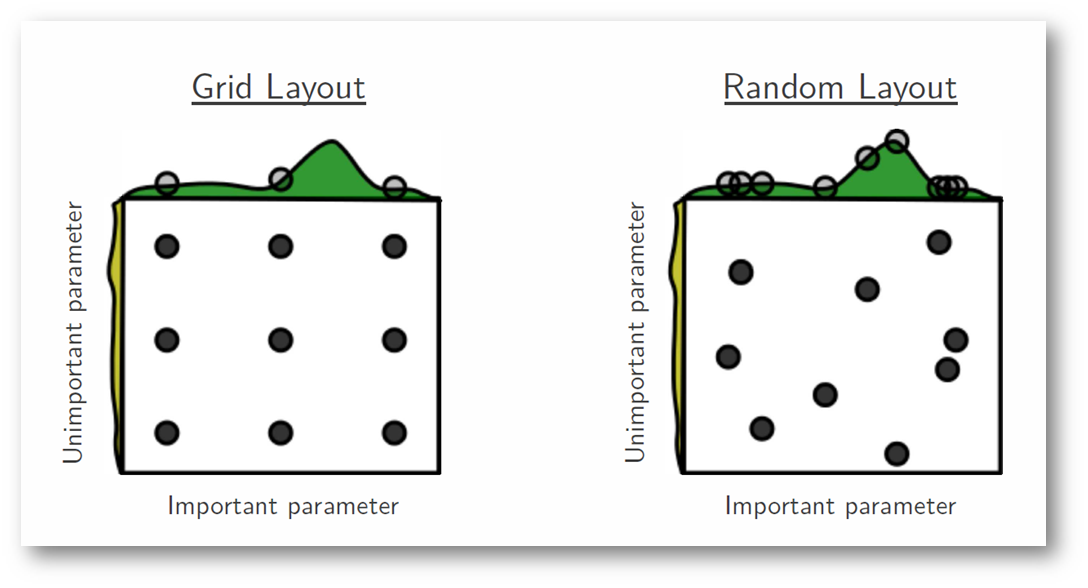
\includegraphics[width = 5.5in]{grid_vs_random.png}
\caption{Grid Search vs Random Search}
\end{center}
\end{figure}
%\begin{align}\label{eqn:22}
%x=2s
%\end{align}
%IN \eqref{eqn:22}, we consider the interaction 



\section{Modeling}

\subsection{CNN Model}

\subsection{Genetic Algorithm}
There many advantages of using genetic algorithm for hyperparameter optimization:
\section{Result}

\section{Conclusion}

\end{document}